\documentclass[a4paper, 11pt, twocolumn]{article}

\usepackage[czech]{babel}
\usepackage[utf8]{inputenc}
\usepackage[IL2]{fontenc}
\usepackage[left=1.5cm, top=2.5cm, text={18cm, 25cm}]{geometry}

\usepackage{times}
\usepackage{amsthm}
\usepackage{amssymb}
\usepackage{amsmath}
\usepackage{stackrel}
\usepackage{graphicx}

\graphicspath{{./img/}}



\begin{document}

	\begin{titlepage}
		\begin{center}
			\begin{center}
			
\includegraphics[scale=0.15]{logo_cz.png} \\
			\end{center}
			\vspace{\stretch{0.382}} 
			\huge {Specifikace zadání a uživatelských požadavků} \\
			\Large {Tvorba uživatelských rozhraní} \\
			\vspace{\stretch{0.618}}
		\end{center}

		\Large{\hfill Vojtěch Kališ (xkalis03)} \\
		\Large{2021 \hfill Jan Lutonský (xluton02)}
	\end{titlepage}
	
	\twocolumn[{\centering{\Large \textbf{Individuální průzkum}\par}
	{\large Vojtěch Kališ, xkalis03@stud.fit.vutbr.cz\par}}
	\par\vspace*{0.8cm}]

	\section*{\large{Téma -- mobilní aplikace Time Planner}}
	\vspace*{-0.2cm}
	Jakožto téma jsem se rozhodl vybrat nějakou aplikaci, jejíž funkcionalita spočívá ve vytváření plánů, upomínek či jakéhokoliv jiného druhu poznámek za
	účelem zapsání si či připomenutí důležité události, schůze, nebo i~trivialit jako co je potřeba koupit při příští návštěvě obchodu apod.; čili jakýkoliv 
	například digitální kalendář, poznámkový blok a~jiné aplikace umožňující výše popsané. Zároveň proběhla snaha najít takovou aplikaci, na níž byly na
	první pohled patrné chyby z~pohledu GUI a~uživatelského procesu, a~to za účelem zjednodušení analýzy problémů dané aplikace a~následného návrhu
	jejich řešení.
	
	\section*{\large{Způsob zkoumání uživatele}}
	\vspace*{-0.2cm}
	Jako subjekt pro svůj uživatelský průzkum jsem si vybral svého bratra, jemuž jsem aplikaci na chvíli předal a~následně jej podrobil několika předem 
	přichystaným stručným otázkám, které měly za účel zjistit jeho pocity z aplikace, připomínky, požadavky a jiné.

	\section*{\large{Požadavky uživatele}} 
	\vspace*{-0.2cm}
	\begin{itemize}
		\item Přehlednost
		\vspace{-0.2cm}
		\item Jednoduchost použití
		\vspace{-0.2cm}
		\item Není zapotřebí převeliké množství funkcí
		\vspace{-0.2cm}
		\item Možnost změny barevného scématu a~pozadí
		\vspace{-0.2cm}
		\item Rychlá editace položek
	\end{itemize}

	\section*{\large{Způsob používání současné aplikace}}
	\vspace*{-0.2cm}
	Momentální aplikace je založena na třídění všech nových i~již vytvořených úloh do skupin podle různých kondicí, převážně pak tedy místa jejich vykonání, 
	čili např. na poznámky vytvořené pro školu, práci, na doma, volný čas a~tak dále. Postrádá možnost zobrazit je všechny chronologicky za sebou a~tím
	zbytečně vytváří zmatek, což jde proti jejímu účelu. Ihned po prvotním spuštění aplikace na uživatele vyskočí několikakrokový tutoriál na vytvoření nové
	úlohy, načež je uživatel stejně zmaten co to vlastně vytvořil a~proč, a~poté navíc zjistí že jej čeká ještě zkouknout dalších 10 tutoriálů. Odhaduji, že 
	právě v~tenhle moment by to obvyklý uživatel vzdal a~aplikaci zavřel, čemuž napovídá i~nepěkné hodnocení aplikace.


	\section*{\large{Identifikované potíže}}
	\vspace*{-0.2cm}
	\begin{itemize}
		\item Aplikace má zbytečně příliš mnoho funkcí, což ji dělá nepřehlednou a~komplikovanou
		\vspace{-0.2cm}
		\item Pouze dvě barevná schémata, skoro žádné možnosti kustomizace
		\vspace{-0.2cm}
		\item Zákazník očekává jednoduché řešení jednoduchého problému, ale čeká na něj složité monstrum
	\end{itemize}

	\section*{\large{\centering Vlastní návrh nového řešení}}
	\vspace*{-0.2cm}
	Aplikace má v hlavním panelu nástrojů pouze tři hlavní funkce, a~to konkrétně funkci pro vytvoření úlohy, zobrazení kalendáře s podrobnostmi k úlohám 
	v~následujících dnech a~také možnost grafického přepnutí mezi více režimy zobrazení úloh, přesně v tomto pořadí. Vytvořené úlohy obsahují v~hlavním 
	menu pouze jejich jméno a~čas konání, přičemž je možná každou úlohu rozkliknout, což otevře textový editor v~němž je možné i~doplnit přiblíženější 
	specifikaci k~dané ploze. V~pravém rohu položky je také tlačítko, které po rozkliknutí otevře jednoduché drop-down menu s možnostmi přejmenování 
	položky, nastavení upomínky a~nebo odstranění položky. V~pravém horním rohu menu je tlačítko jejž rozkliknutí otevře Nastavení, kde je dále 
	umožněno například měnit barevné schéma aplikace výběrem z~RGB palety, změnit používaný jazyk, nastavení zvuku apod.
	\vspace*{-0.1cm}
	\begin{center}
	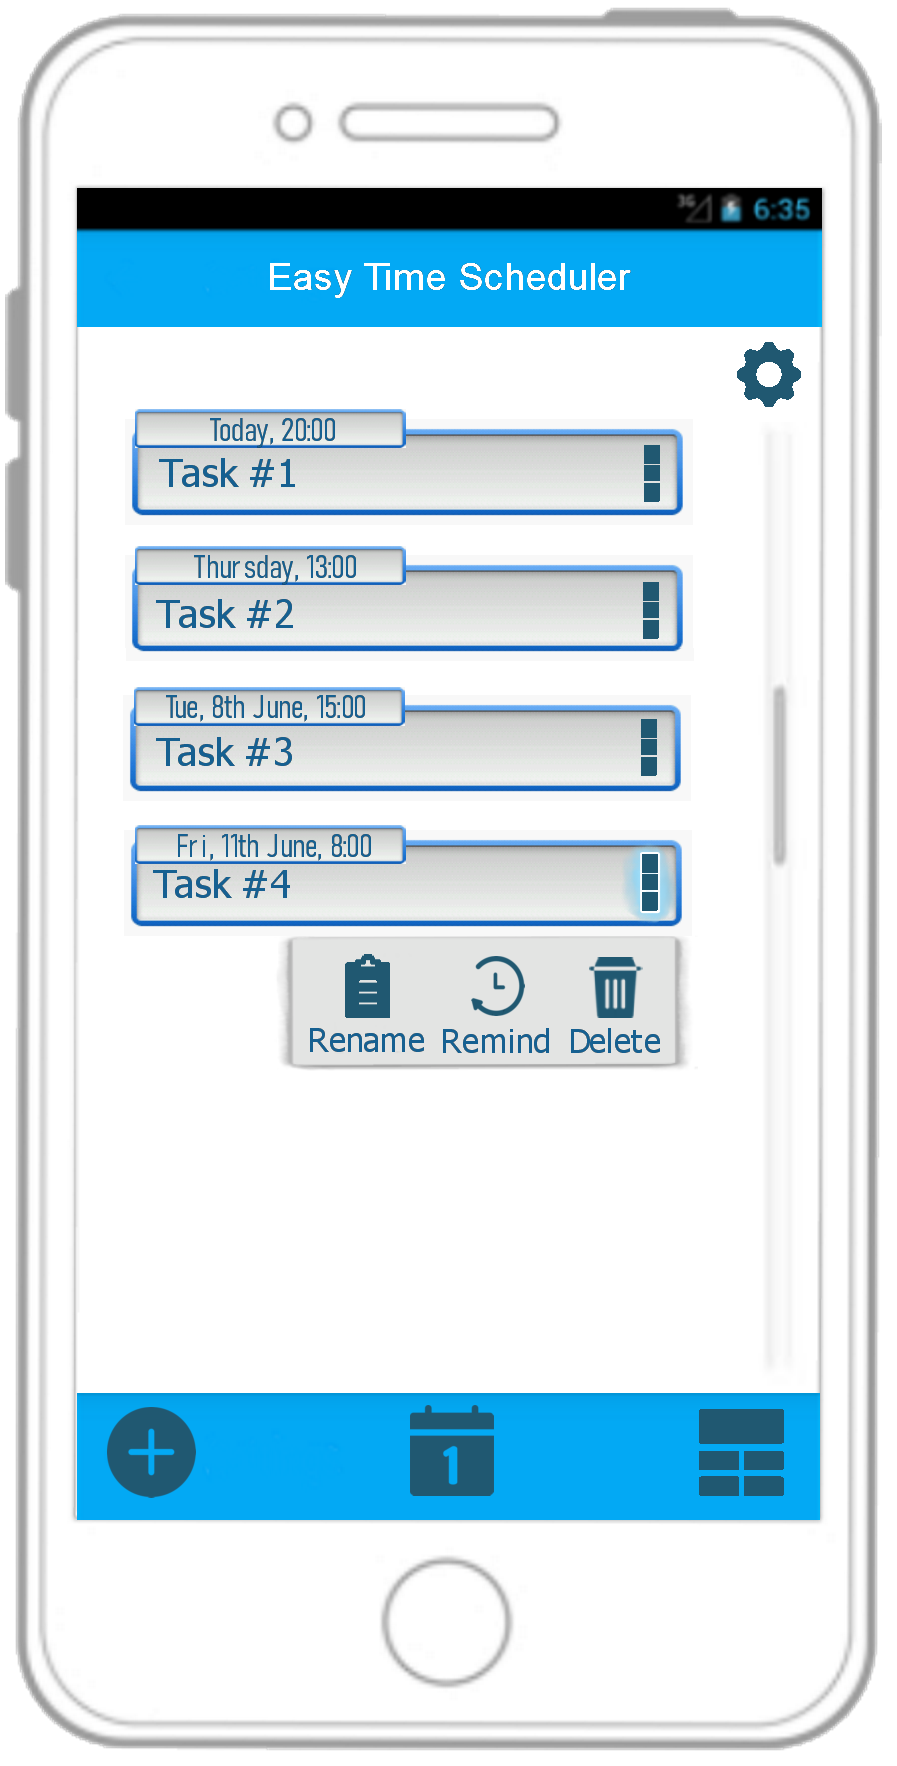
\includegraphics[width=0.34\textwidth]{timeplanner.png}
	\end{center}

	\newpage


	\twocolumn[{\centering{\Large \textbf{Individuální průzkum}\par}
	{\large Jan Lutonský, xluton02@stud.fit.vutbr.cz\par}}
	\par\vspace*{0.8cm}]

	\section*{\large{Téma -- školní administrativní systém}}
	\vspace*{-0.2cm}
 	Při hledání témat projektu jsem se ptal lidí v mém okolí jestli neznají nějaké aplikace, které by podle nich potřebovali zlepšit a každý kterého jsem se zeptal 
	našel alespoň jednu aplikaci která by potřebovala redesign. Ze všech byla ale nejhorší aplikace pro správu informací o studentech, učitelích a majetku školy 
	jedné nejmenované hudební školy. Proto jsem se rozhodl že se pokusím systém vylepšit ve svém projektu.
	
	\section*{\large{Sledování uživatele}}
	\vspace*{-0.2cm}
	Sledoval jsem uživatele při práci s jejich dosavadním administračním systémem, bylo zjevné že nejsou se systémem vůbec spokojeni. systém je příliš složitý 
	pro běžnou kancelářskou práci.

	\section*{\large{Uživatelé systému}}
	\vspace*{-0.2cm}
	Se systémem pracují dvě skupiny uživatel, administrační pracovníci a učitelé, kteří ve škole učí. Administrační pracovníci mají zkušenosti s prací na počítači a 
	většínu dne tráví editací údajů v systému. Učitelé na druhou stranu jsou většinou starší lidé a mají problém při práci s počítačem proto si zvykli se systémem 
	nepracovat vůbec a veškerou svou práci převedly na administrativní pracovníky. Učitelé ze systému potřebují číst informace o rozvrhu, seznamy žáku a 
	kontaktní informace na rodiče a popřípadě zadávat známky ke konkrétnímu žákovi.

	\section*{\large{Požadavky uživatele}}
	\vspace*{-0.2cm}
	\begin{itemize}
		\item Snadná manipulace se systémem, eliminace manuálního vypisování známých informací
		\vspace{-0.2cm}
		\item Snadné vyhledávání informací a jejich filtrování
		\vspace{-0.2cm}
		\item Snadné tisknutí informací na tiskárně
		\vspace{-0.2cm}
		\item Implementovat historii úpravy systému, možná reverzace akcí
		\vspace{-0.2cm}
		\item Zjednodušené rozhraní pro učitele
	\end{itemize}

	\section*{\large{Způsob používání současné aplikace}}
	\vspace*{-0.2cm}
	Systém slouží pro vyhledávání studentů a modifikace informací o nich například školné, předměty které navštěvují, do jaké pobočky dochází, známky, 
	atd.. A k generování informací nutných pro práci učitelů: rozvrhy, seznamy žáků, vysvědčení. \\

   	\noindent Sepsal jsem jednotlivé kroky které uživatel musí podstoupit při změně školného jednoho žáka. \\

   	\textit{Změna školného žáka}
	\vspace*{-0.2cm}

   	\begin{enumerate}
        \item  uživatel musí stisknout tlačítko studenti a vyhledat jméno žáka
        \vspace*{-0.2cm}
        \item  v seznamu stejných jmen najít správného žáka manuálním porovnáváním čísla studenta
        \vspace*{-0.2cm}
        \item  po té co byl vybrán správný žák je nutno stisknout tlačítko upravit
        \vspace*{-0.2cm}
        \item  dále je nutné manuálně vypočíst a manuálně vepsat školné, toto školné je možno vypočíst z informací uložených v systému automaticky
        \vspace*{-0.2cm}
        \item  zmáčknout tlačítko uložit nebo tlačítko zavřít, tyto tlačítka provádí stejnou akci
        \vspace*{-0.2cm}
        \item  zmáčknout tlačítko faktury u žáka a tlačítko opravit dále kliknout na tlačítko řádky
        \vspace*{-0.2cm}
        \item  manuálně upravit řádek cena, stejná hodnota jako školné, které bylo vyplněno v kroku 4)
        \vspace*{-0.2cm}
        \item  zmáčknout tlačítko uložit nebo tlačítko zavřít
        \vspace*{-0.2cm}
        \item  stáhnout fakturu a odeslat mailem
        \vspace*{-0.2cm}
   	\end{enumerate}
	
	\vspace*{0.2cm}
   	\textit{Tento postup by mohl vypadat následovně}
	\vspace*{0.2cm}
	
   	\begin{enumerate}
        \item zmáčknout tlačítko osoby
        \vspace{-0.2cm}
        \item vyhledat podle čísla žáka konkrétního žáka
        \vspace{-0.2cm}
        \item  upravit informace o studiu, které automaticky změní cenu školného
        \vspace{-0.2cm}
        \item  zmáčknout tlačítko vygenerovat fakturu, které vygeneruje fakturu v pdf
        \vspace{-0.2cm}
        \item  odeslat pdf mailem
        \vspace{-0.2cm}
   	\end{enumerate}

	\newpage

	\section*{\large{Vlastní návrh nového řešení}}
	\vspace*{-0.2cm}
	Hlavním cílem je zjednodušit a zpříjemnit práci administračním pracovníkům a to tak že sjednotím podsystémy. Implementuji historii změn v systému 
	aby bylo možné měnit chyby a vytvořit nový přívětivější podsystém pro učitele.

	\begin{center}
	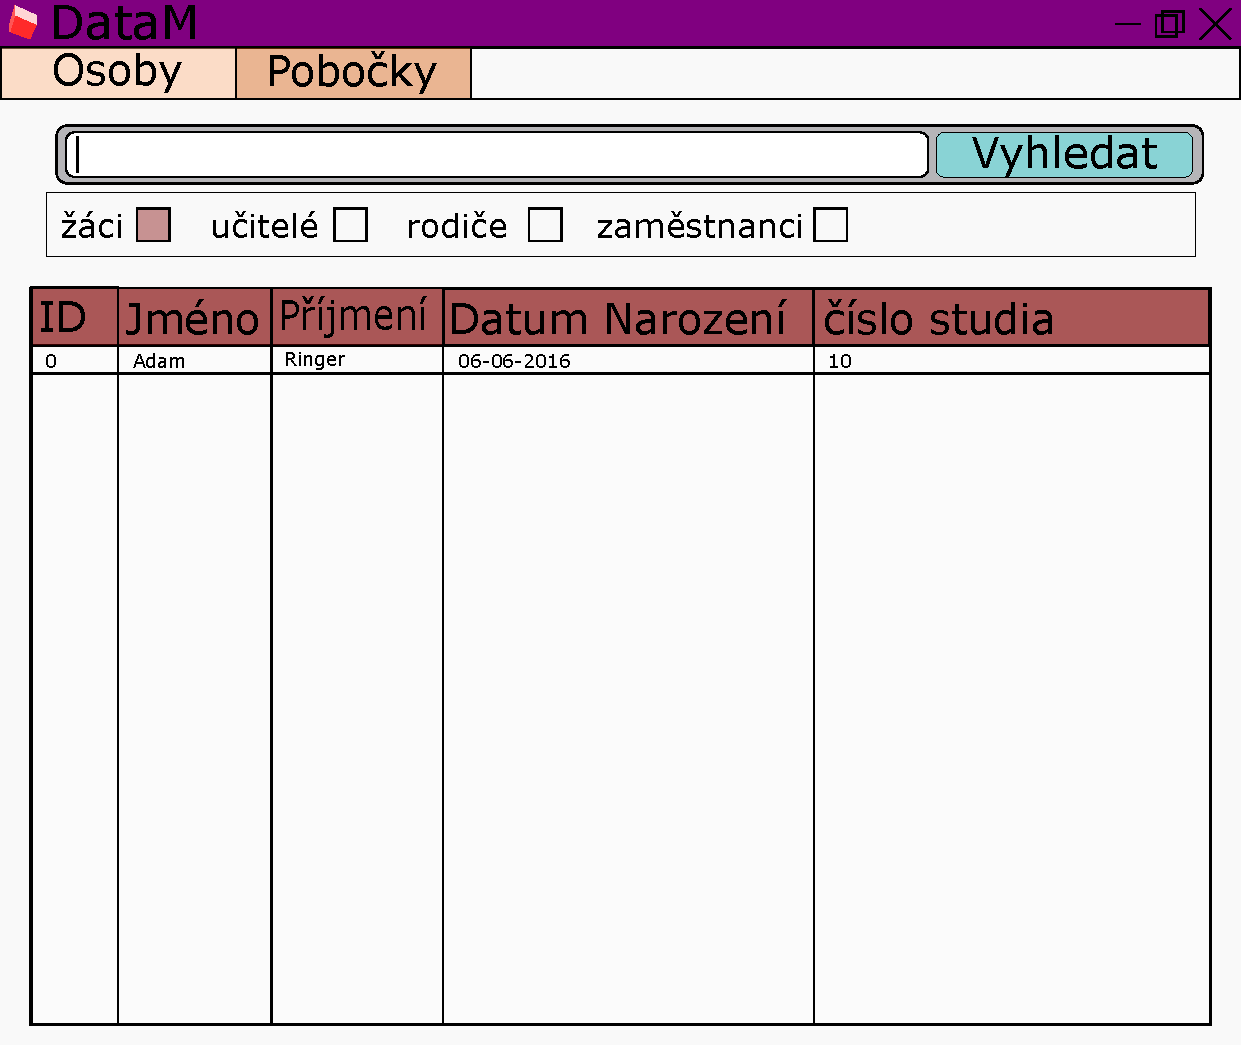
\includegraphics[width=0.5\textwidth]{GUI.pdf}
	\end{center}


	\newpage


	\twocolumn[{\centering{\huge \textbf{Specifikace zadání a uživatelských požadavků}\par}
	{\Large téma Školní administrativní systém\par}}
	\par\vspace*{0.8cm}

	
	\section*{\large{Důvod výběru tématu}}
	\vspace*{-0.2cm}
	Téma ,,Školní administrativní systém`` jsme se rozhodli vybrat hned z několika důvodů, a to větší škály možností v oblasti implementace různých 
	vylepšení, zajímavosti daného tématu, a v neposlední řadě také jelikož druhé téma se nám v porovnání zdálo až příliš primitivní.

	\section*{\large{Analýza uživatele}}
	\vspace*{-0.2cm}
	Uživatelem aplikace je učitel nebo administrativní pracovník, který aplikaci používá k zobrazování a/nebo modifikaci informací o studentech, 
	zaměstnancích školy, majetku školy a studijních programech. 

	\section*{\large{Potřeby uživatele}}
	\vspace*{-0.2cm}
	Uživatel potřebuje co nejjednodušší grafické rozhraní pro učitele a automatizaci pro administrativní pracovníky do níž by bylo možné vkládat informace a 
	poté je nazpět číst. Preferována je funkčnost a přehlednost, ovšem nebylo by od věci zařídit i vizualisticky uspokojivý vzhled; ne však na úkor 
	přehlednosti. Dále je kladen důraz na efektivní tisk informací a sdílení informací přes mail.

	\section*{\large{Popis současného řešení}}
	\vspace*{-0.2cm}]
	\begin{center}
	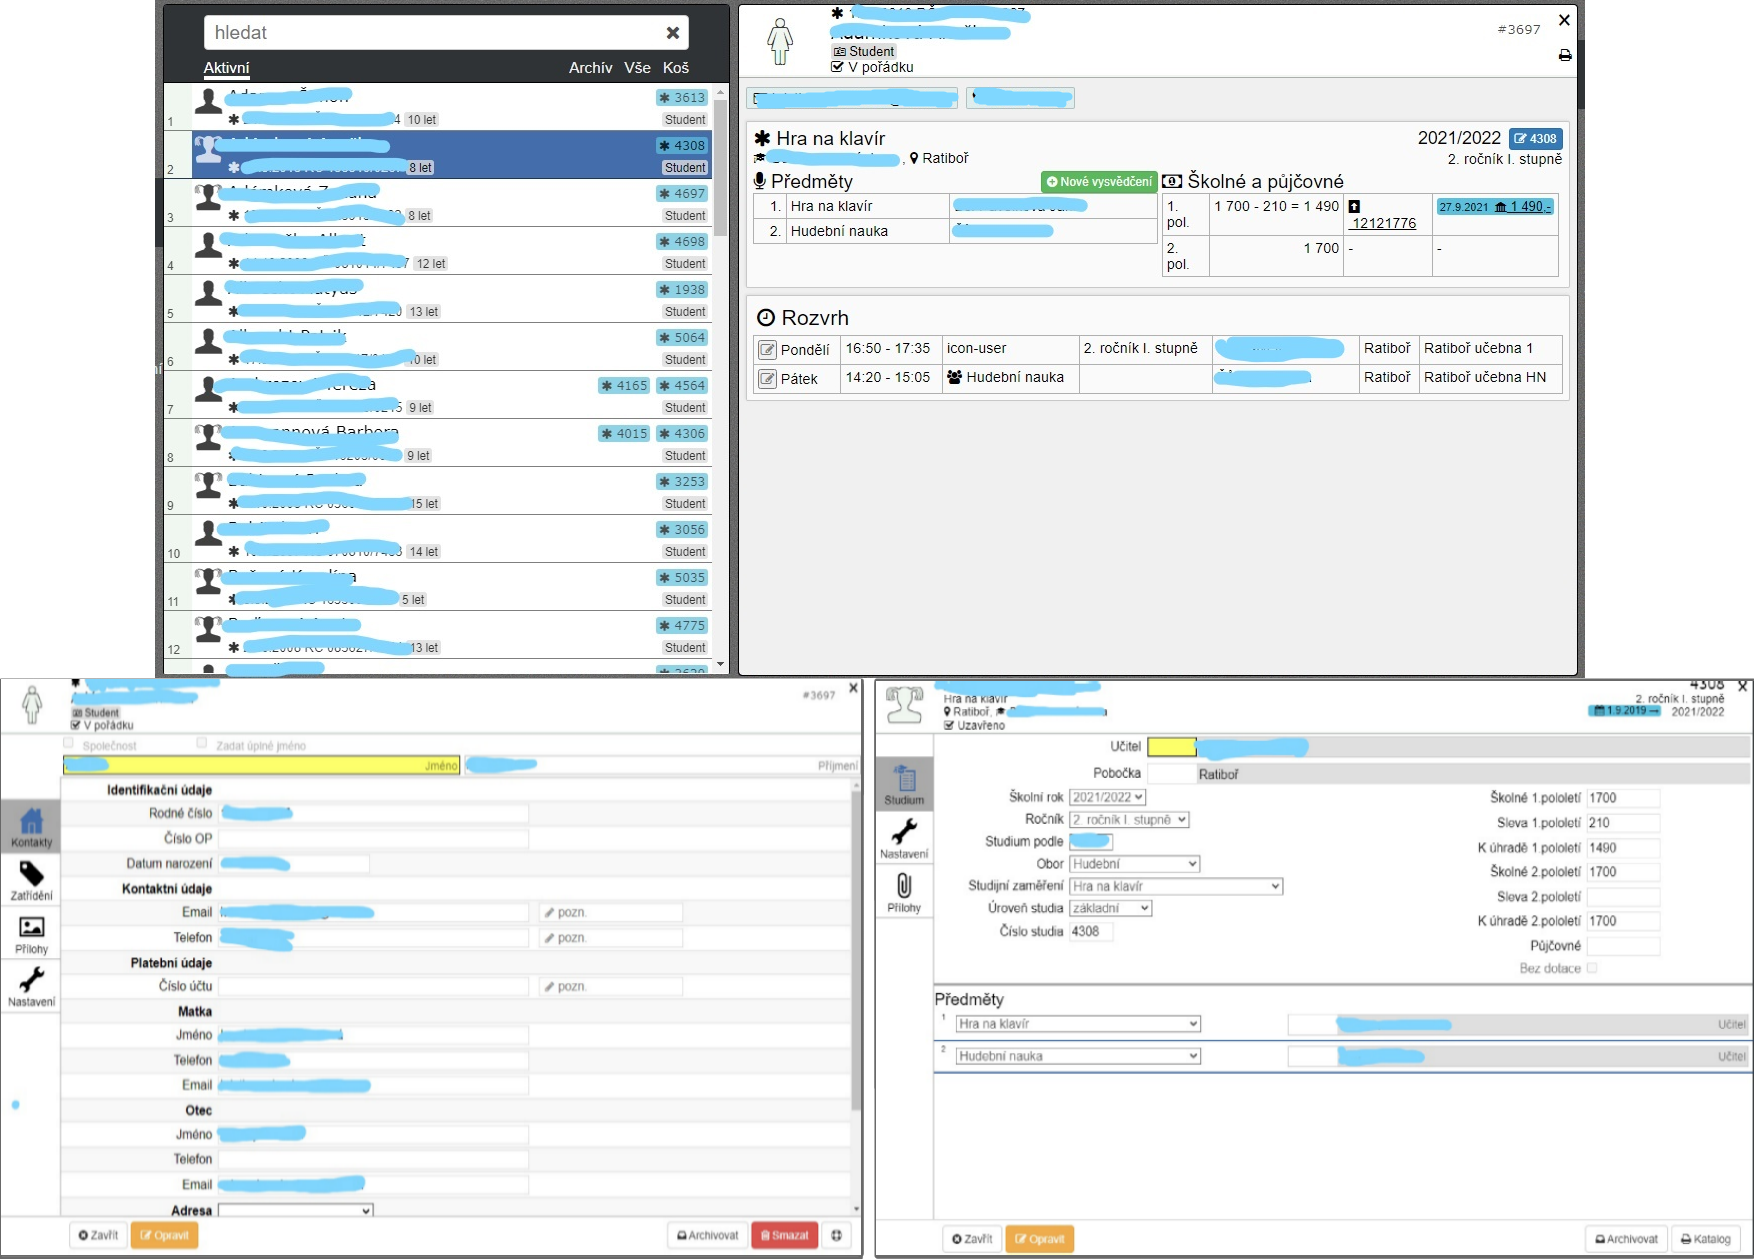
\includegraphics[width=1\textwidth]{puvodni.png}
	\end{center}

	\twocolumn[
	\section*{\large{Návrh zadání}}
	\vspace*{-0.2cm}
	Proběhne snaha implementace sjednocení co nejvíce podsystémů do jednoho (ne však na úkor přehlednosti),  automatizace vypisování již předem 
	známých nebo vypočítatelných položek, jednoduššího a srozumitelnějšího vyhledávání žáků, snadněji navigovatelného uživatelského rozhraní, a v 
	neposlední řadě také možnosti zobrazení historie změn a jejich případné reverzaci. Uživateli tak bude umožněno systém využívat efektivněji, bude mít 
	přístup k více možnostem načtení a editace informací, a k vykonání potřebných změn mu bude stačit značně menší počet manuálních kroků.

	\noindent Konkrétní příklad úpravy a zjednodušení uživatelského procesu lze nalézt v Individuálním průzkumu tohohle tématu, strana 2, sekce Způsob 
	používání současné aplikace. Je zde patrná snaha o zmenšení počtu nutně vykonávaných kroků ze strany uživatele pro zařízení jednoho konkrétního 
	výstupu.

	\section*{\large{Návrh řešení (předběžný)}}
	\vspace*{-0.2cm}]
	\begin{center}
	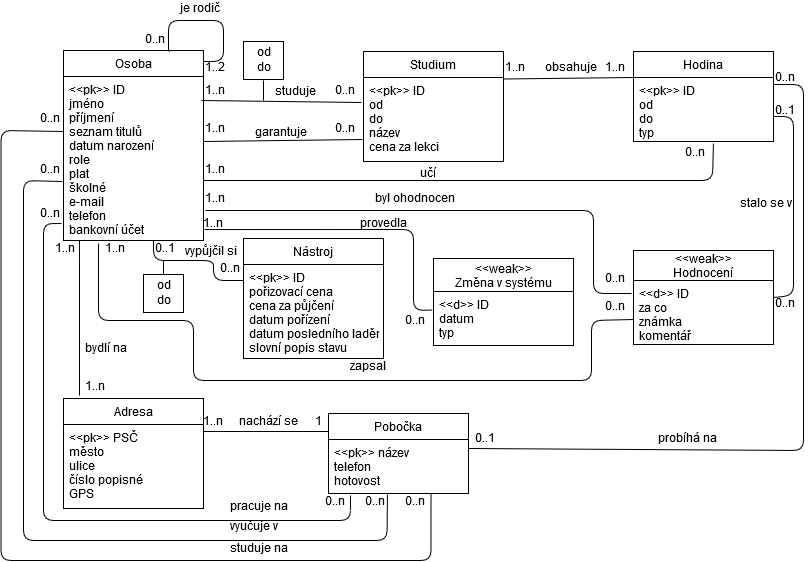
\includegraphics[width=1\textwidth]{UML.png}
	\end{center}

	\clearpage


	\twocolumn[{\centering{\huge \textbf{API}\par}
	{\Large Popis rozhraní systému\par}}
	\par\vspace*{0.8cm}]

\section{Vstupní funkce}\label{vstupnuxed-funkce}

\subsection{add\_person}\label{addux5fperson}
\vspace*{-0.3cm}
funkce přijme informace o osobě zabalené do objektu a pokusí se je vložit do systému. \\
\noindent \underline{\textbf{vstupy:}} \, objekt popisující osobu  \\
\noindent \underline{\textbf{výstupy:}} \, \textit{bool} -- \textbf{true} povedlo se přidat \\
\hspace*{2.35cm} -- \textbf{false} nepovedlo se přidat  \\
\underline{\textbf{Možné chyby:}} chyba databáze \\
\hspace*{1.4cm} nekorektní informace o uživateli

\subsection{add\_instrument}\label{addux5finstrument}
\vspace*{-0.3cm}
funkce příjme informace o hudebním nástroji zabalené do objektu a pokusí se je vložit do systému. \\
\noindent \underline{\textbf{vstupy:}} \, objekt popisující hudební nástroj  \\
\noindent \underline{\textbf{výstupy:}} \, \textit{bool} -- \textbf{true} povedlo se přidat \\
\hspace*{2.35cm} -- \textbf{false} nepovedlo se přidat  \\
\underline{\textbf{Možné chyby:}} chyba databáze \\
\hspace*{1.4cm} nekorektní informace o hudebním nástroji

\subsection{add\_studium}\label{addux5fstudium}
\vspace*{-0.3cm}
funkce se pokusí přidat nové studium popsané objektem do systému. \\
\noindent \underline{\textbf{vstupy:}} \, objekt popisující studium  \\
\noindent \underline{\textbf{výstupy:}} \, \textit{bool} -- \textbf{true} povedlo se přidat \\
\hspace*{2.35cm} -- \textbf{false} nepovedlo se přidat  \\
\underline{\textbf{Možné chyby:}} chyba databáze \\
\hspace*{1.4cm} nekorektní informace o studiu

\subsection{add\_address}\label{addux5faddress}
\vspace*{-0.3cm}
funkce se pokusí přidat novou adresu do systému. \\
\noindent \underline{\textbf{vstupy:}} \, objekt popisující adresu  \\
\noindent \underline{\textbf{výstupy:}} \, \textit{bool} -- \textbf{true} povedlo se přidat \\
\hspace*{2.35cm} -- \textbf{false} nepovedlo se přidat  \\
\underline{\textbf{Možné chyby:}} chyba databáze \\
\hspace*{1.4cm} nekorektní informace o adrese

\subsection{add\_branch\_office}\label{addux5fbranchux5foffice}
\vspace*{-0.3cm}
funkce se pokusí přidat novou pobočku do systému. \\
\noindent \underline{\textbf{vstupy:}} \, objekt popisující pobočku  \\
\noindent \underline{\textbf{výstupy:}} \, \textit{bool} -- \textbf{true} povedlo se přidat \\
\hspace*{2.35cm} -- \textbf{false} nepovedlo se přidat  \\
\underline{\textbf{Možné chyby:}} chyba databáze \\
\hspace*{1.4cm} nekorektní informace o pobočce


\newpage


\subsection{person\_rent\_instrument}\label{personux5frentux5finstrument}
\vspace*{-0.3cm}
vytvoří záznam o půjčení hudebního nástroje osobou. \\
\noindent \underline{\textbf{vstupy:}} \, objekt popisující osobu  \\
\noindent \hspace*{1.4cm} objekt popisující hudební nástroj  \\
\noindent \hspace*{1.4cm} objekt popisující půjčku  \\
\noindent \underline{\textbf{výstupy:}} \, \textit{bool} -- \textbf{true} povedlo se přidat \\
\hspace*{2.35cm} -- \textbf{false} nepovedlo se přidat  \\
\underline{\textbf{Možné chyby:}} chyba databáze \\
\hspace*{1.4cm} nekorektní informace o vstupech

\subsection{rate\_student}\label{rateux5fstudent}
\vspace*{-0.3cm}
vytvoří hodnocení studenta učitelem. \\
\noindent \underline{\textbf{vstupy:}} \, objekt popisující osobu student  \\
\noindent \hspace*{1.4cm} objekt popisující osobu učitel  \\
\noindent \hspace*{1.4cm} objekt popisující hodnocení studenta  \\
\noindent \underline{\textbf{výstupy:}} \, \textit{bool} -- \textbf{true} povedlo se přidat \\
\hspace*{2.35cm} -- \textbf{false} nepovedlo se přidat  \\
\underline{\textbf{Možné chyby:}} chyba databáze \\
\noindent\hspace*{1.4cm} objekt studenta není student \\
\hspace*{1.4cm} objekt učitele není učitel \\
\hspace*{1.4cm} chybné vstupní informace \\

\section{Nastavovací funkce}\label{nastavovacuxed-funkce}

\subsection{studium\_set\_students}\label{studiumux5fsetux5fstudents}
\vspace*{-0.3cm}
přidělí množinu žáků ke studiu. \\
\noindent \underline{\textbf{vstupy:}} \, množina žáků  \\
\noindent \hspace*{1.4cm} množina žáků \\
\noindent \hspace*{1.4cm} množina studií  \\
\noindent \underline{\textbf{výstupy:}} \, \textit{bool} -- \textbf{true} povedlo se \\
\hspace*{2.35cm} -- \textbf{false} nepovedlo se  \\
\underline{\textbf{Možné chyby:}} prázdná množina žáků nebo studií

\subsection{studium\_set\_lectures}\label{studiumux5fsetux5flectures}
\vspace*{-0.3cm}
přidělí dané vyučovací hodiny k danému studiu. \\
\noindent \underline{\textbf{vstupy:}} \, množina vyučovacích hodin  \\
\noindent \hspace*{1.4cm} množina studií \\
\noindent \underline{\textbf{výstupy:}} \, \textit{bool} -- \textbf{true} povedlo se \\
\hspace*{2.35cm} -- \textbf{false} nepovedlo se  \\
\underline{\textbf{Možné chyby:}} prázdná množina hodin nebo studií
\vfill


\pagebreak


\section{Aktualizační funkce}\label{aktualizaux10dnuxed-funkce}

\subsection{end\_rent\_instrument}\label{endux5frentux5finstrument}
\vspace*{-0.3cm}
ukončí vypůjčení hudebního nástroje. \\
\noindent \underline{\textbf{vstupy:}} \, záznam o půjčení nástroje  \\
\noindent \hspace*{1.4cm} stav nástroje \\
\noindent \underline{\textbf{výstupy:}} \, \textit{bool} -- \textbf{true} povedlo se \\
\hspace*{2.35cm} -- \textbf{false} nepovedlo se  \\
\underline{\textbf{Možné chyby:}} chyba databáze \\
\hspace*{1.4cm} prázdná množina hodin nebo studií \\

\subsection{update}\label{update}
\vspace*{-0.3cm}
přepočítá všchny hodnoty v databázi, co dává smysl přepočítat. \\
\noindent \underline{\textbf{vstupy:}} \, --  \\
\noindent \underline{\textbf{výstupy:}} \, \textit{bool} -- \textbf{true} povedlo se \\
\hspace*{2.35cm} -- \textbf{false} nepovedlo se  \\
\underline{\textbf{Možné chyby:}} chyba databáze



\section{Tvořící funkce}\label{tvoux159uxedcuxed-funkce-funkce}

\subsection{generate\_classification}\label{generateux5fclassification}
\vspace*{-0.3cm}
vygeneruje vysvědčení pro skupinu žáků z jednoho studia a uloží je jako PDF. \\
\noindent \underline{\textbf{vstupy:}} \, množina studentů  \\
\noindent \hspace*{1.4cm} studium \\
\noindent \underline{\textbf{výstupy:}} \, \textit{bool} -- \textbf{true} povedlo se \\
\hspace*{2.35cm} -- \textbf{false} nepovedlo se  \\
\underline{\textbf{Možné chyby:}} chyba databáze \\
\hspace*{1.4cm} jedna nebo více osob z množiny studentů není \\
\hspace*{2cm} student \\
\hspace*{1.4cm} jedna nebo více osob z množiny studentů není 
\hspace*{2cm} zapsána na dané studium \\
\hspace*{1.4cm} chyba převodu informací do pdf

\subsection{generate\_tuition\_bill}\label{generateux5ftuitionux5fbill}
\vspace*{-0.3cm}
vygeneruje fakturu za školné pro množinu žáků a uloží je jako PDF. \\
\noindent \underline{\textbf{vstupy:}} \, množina žáků  \\
\noindent \hspace*{1.4cm} studium \\
\noindent \underline{\textbf{výstupy:}} \, \textit{bool} -- \textbf{true} povedlo se \\
\hspace*{2.35cm} -- \textbf{false} nepovedlo se  \\
\underline{\textbf{Možné chyby:}} chyba databáze \\
\hspace*{1.4cm} jedna nebo více osob z množiny studentů není \\
\hspace*{2cm} student \\
\hspace*{1.4cm} chyba převodu informací do pdf

\vfill

\subsection{generate\_salaries}\label{generateux5fsalaries}
vygeneruje výplaty a uloží je jako PDF. \\
\noindent \underline{\textbf{vstupy:}} \, množina zaměstnanců  \\
\noindent \hspace*{1.4cm} studium \\
\noindent \underline{\textbf{výstupy:}} \, \textit{bool} -- \textbf{true} povedlo se \\
\hspace*{2.35cm} -- \textbf{false} nepovedlo se  \\
\underline{\textbf{Možné chyby:}} chyba databáze \\
\hspace*{1.4cm} jedna nebo více osob z množiny zaměstnanců není \\
\hspace*{2cm} zaměstnanec \\
\hspace*{1.4cm} chyba při vytváření PDF

\subsection{generate\_schedule}\label{generateux5fschedule}
\vspace*{-0.3cm}
vygeneruje rozvrh studentů jako PDF. \\
\noindent \underline{\textbf{vstupy:}} \, množina studentů  \\
\noindent \hspace*{1.4cm} studium \\
\noindent \underline{\textbf{výstupy:}} \, \textit{bool} -- \textbf{true} povedlo se \\
\hspace*{2.35cm} -- \textbf{false} nepovedlo se  \\
\underline{\textbf{Možné chyby:}} chyba databáze \\
\hspace*{1.4cm} jedna nebo více osob z množiny studentů není \\
\hspace*{2cm} student \\
\hspace*{1.4cm} chyba při vytváření PDF


\section{Odstraňovací funkce}\label{odstraux148ovacuxed-funkce}


\subsection{remove\_person}
\vspace*{-0.3cm}
odstraní záznam o osobě ze systému. \\
\noindent \underline{\textbf{vstupy:}} \, množina osob  \\
\noindent \underline{\textbf{výstupy:}} \, \textit{bool} -- \textbf{true} povedlo se \\
\hspace*{2.35cm} -- \textbf{false} nepovedlo se  \\
\underline{\textbf{Možné chyby:}} chyba databáze

\subsection{remove\_instrument}
\vspace*{-0.3cm}
odstraní záznam o hudebním nástroji ze systému ze systému. \\
\noindent \underline{\textbf{vstupy:}} \, množina nástrojů  \\
\noindent \underline{\textbf{výstupy:}} \, \textit{bool} -- \textbf{true} povedlo se \\
\hspace*{2.35cm} -- \textbf{false} nepovedlo se  \\
\underline{\textbf{Možné chyby:}} chyba databáze

\subsection{remove\_studium}
\vspace*{-0.3cm}
odstraní záznam o studiu ze systému ze systému. \\
\noindent \underline{\textbf{vstupy:}} \, množina nástrojů  \\
\noindent \underline{\textbf{výstupy:}} \, \textit{bool} -- \textbf{true} povedlo se \\
\hspace*{2.35cm} -- \textbf{false} nepovedlo se  \\
\underline{\textbf{Možné chyby:}} chyba databáze
\vfill


\pagebreak


\subsection{remove\_addres}
\vspace*{-0.3cm}
odstraní záznam o adrese ze systému ze systému. \\
\noindent \underline{\textbf{vstupy:}} \, množina nástrojů  \\
\noindent \underline{\textbf{výstupy:}} \, \textit{bool} -- \textbf{true} povedlo se \\
\hspace*{2.35cm} -- \textbf{false} nepovedlo se  \\
\underline{\textbf{Možné chyby:}} chyba databáze

\subsection{remove\_branch\_office}
\vspace*{-0.3cm}
odstraní záznam o pobočce ze systému ze systému. \\
\noindent \underline{\textbf{vstupy:}} \, množina nástrojů  \\
\noindent \underline{\textbf{výstupy:}} \, \textit{bool} -- \textbf{true} povedlo se \\
\hspace*{2.35cm} -- \textbf{false} nepovedlo se  \\
\underline{\textbf{Možné chyby:}} chyba databáze


\section{práce s historií}


\subsection{get\_history}
\vspace*{-0.3cm}
vrátí seznam změn podle filtru. \\
\noindent \underline{\textbf{vstupy:}} \, filtr  \\
\noindent \underline{\textbf{výstupy:}} \, množina změn\\
\underline{\textbf{Možné chyby:}} chyba databáze \\
\hspace*{1.4cm} špatný filtr\\

\subsection{try\_undo}
\vspace*{-0.3cm}
Pokusí se o odělání změny \\
\noindent \underline{\textbf{vstupy:}} \, změna  \\
\noindent \underline{\textbf{výstupy:}} \, \textit{bool} -- \textbf{true} povedlo se \\
\hspace*{2.35cm} -- \textbf{false} nepovedlo se  \\
\underline{\textbf{Možné chyby:}} chyba databáze \\
\hspace*{1.4cm} změnu nelze vrátit\\


\section{získávání informací}


\subsection{quarry\_person}
\vspace*{-0.3cm}
Vyhledá osobu v databázy. \\
\noindent \underline{\textbf{vstupy:}} \, filtr  \\
\noindent \underline{\textbf{výstupy:}} \, množina osob \\
\underline{\textbf{Možné chyby:}} chyba databáze \\

\subsection{quarry\_instrument}
\vspace*{-0.3cm}
Vyhledá hudební nástroje v databázy . \\
\noindent \underline{\textbf{vstupy:}} \, filtr \\
\noindent \underline{\textbf{výstupy:}} \, množina hudebních nástrojů\\
\underline{\textbf{Možné chyby:}} chyba databáze \\

\subsection{quarry\_studium}
\vspace*{-0.3cm}
Vyhledá studium v databázy. \\
\noindent \underline{\textbf{vstupy:}} \,  filtr \\
\noindent \underline{\textbf{výstupy:}} \, množina studii \\
\underline{\textbf{Možné chyby:}} chyba databáze \\

\subsection{quarry\_addres}
\vspace*{-0.3cm}
Vyhledá adresu v databazy. \\
\noindent \underline{\textbf{vstupy:}} \, filtr \\
\noindent \underline{\textbf{výstupy:}} \, množina adress   \\
\underline{\textbf{Možné chyby:}} chyba databáze \\

\subsection{quarry\_branch\_office}
\vspace*{-0.3cm}
Vyhledá pobočku v databázy. \\
\noindent \underline{\textbf{vstupy:}} \, filtr  \\
\noindent \underline{\textbf{výstupy:}} \, množina poboček\\
\underline{\textbf{Možné chyby:}} chyba databáze \\
\hfill

\end{document}